\subsection*{Partie A}

On a :
\[
P(A)=0,60,\qquad P(B)=0,12,\qquad P(C)=1-0,60-0,12=0,28.
\]
De plus :
\[
P_A(T)=0,90,\quad P_B(T)=0,95,\quad P_C(T)=0,85.
\]
Donc :
\[
P_A(\overline T)=0,10,\quad P_B(\overline T)=0,05,\quad P_C(\overline T)=0,15.
\]

\begin{enumerate}
	\item L'arbre complété est le suivant :

	\begin{center}
		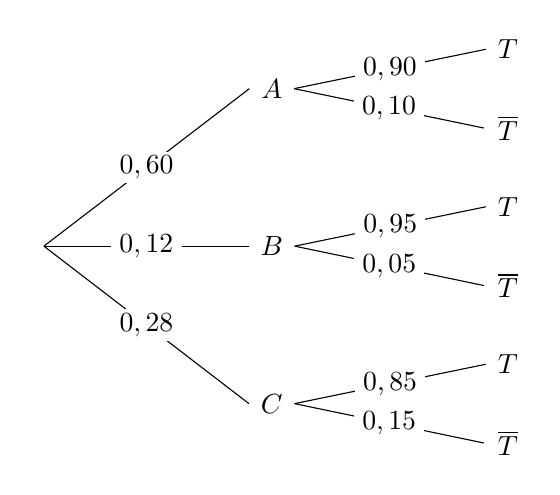
\begin{tikzpicture}[xscale=1,yscale=1]
			\tikzstyle{noeud}=[fill=white,circle,inner sep=2pt]
			\tikzstyle{feuille}=[fill=white,circle,inner sep=2pt]
			\tikzstyle{etiquette}=[midway,fill=white, inner xsep=3pt, inner ysep=1.5pt]
			\def\DistanceInterNiveaux{3}
			\def\DistanceInterFeuilles{1}
			\def\NiveauA{(0)*\DistanceInterNiveaux}
			\def\NiveauB{(1)*\DistanceInterNiveaux}
			\def\NiveauC{(2)*\DistanceInterNiveaux}
			\def\InterFeuilles{(-1)*\DistanceInterFeuilles}
			\node[noeud] (R) at ({\NiveauA},{(2.5)*\InterFeuilles}) {$$};
			\node[noeud] (Ra) at ({\NiveauB},{(0.5)*\InterFeuilles}) {$A$};
			\node[feuille] (Raa) at ({\NiveauC},{(0)*\InterFeuilles}) {$T$};
			\node[feuille] (Rab) at ({\NiveauC},{(1)*\InterFeuilles}) {$\overline{T}$};
			\node[noeud] (Rb) at ({\NiveauB},{(2.5)*\InterFeuilles}) {$B$};
			\node[feuille] (Rba) at ({\NiveauC},{(2)*\InterFeuilles}) {$T$};
			\node[feuille] (Rbb) at ({\NiveauC},{(3)*\InterFeuilles}) {$\overline{T}$};
			\node[noeud] (Rc) at ({\NiveauB},{(4.5)*\InterFeuilles}) {$C$};
			\node[feuille] (Rca) at ({\NiveauC},{(4)*\InterFeuilles}) {$T$};
			\node[feuille] (Rcb) at ({\NiveauC},{(5)*\InterFeuilles}) {$\overline{T}$};
			\draw (R.east)--(Ra.west) node[etiquette] {$0,60$};
			\draw (Ra.east)--(Raa.west) node[etiquette] {$0,90$};
			\draw (Ra.east)--(Rab.west) node[etiquette] {$0,10$};
			\draw (R.east)--(Rb.west) node[etiquette] {$0,12$};
			\draw (Rb.east)--(Rba.west) node[etiquette] {$0,95$};
			\draw (Rb.east)--(Rbb.west) node[etiquette] {$0,05$};
			\draw (R.east)--(Rc.west) node[etiquette] {$0,28$};
			\draw (Rc.east)--(Rca.west) node[etiquette] {$0,85$};
			\draw (Rc.east)--(Rcb.west) node[etiquette] {$0,15$};
		\end{tikzpicture}
	\end{center}

	\item On calcule :
	\[
	P\left(A\cap\overline T\right)=P(A)\times P_A(\overline T)=0,60\times 0,10=0,06.
	\]
	Ainsi, la probabilité que la lame testée provienne du fournisseur A et ne soit pas conforme est égale à $0,06$, soit $6~\%$.

	\item Les évènements $A$, $B$ et $C$ forment une partition de l'univers : une lame provient d'un et un seul des trois fournisseurs.

	D'après la formule des probabilités totales :
	\[
	\begin{aligned}
	P(T)&=P(A\cap T)+P(B\cap T)+P(C\cap T)\\
	&=0,60\times 0,90+0,12\times 0,95+0,28\times 0,85\\
	&=0,54+0,114+0,238\\
	&=0,892.
	\end{aligned}
	\]
	La probabilité que la lame testée soit conforme est donc bien égale à $0,892$.

	\item On cherche $P_{\overline T}(B)$.
	Comme $P(\overline T)=1-0,892=0,108$, on obtient :
	\[
	P_{\overline T}(B)=\dfrac{P(B\cap\overline T)}{P(\overline T)}
	=\dfrac{0,12\times 0,05}{0,108}
	=\dfrac{0,006}{0,108}
	\approx 0,056.
	\]
	Sachant que la lame testée n'est pas conforme, la probabilité qu'elle provienne du fournisseur B est environ égale à $0,056$.
\end{enumerate}

\subsection*{Partie B}

On considère $X$ le nombre de lames non conformes dans un échantillon de 75 lames.

\begin{enumerate}
	\item Pour chaque lame testée, l'expérience aléatoire a deux issues :
	\begin{itemize}[label={\textbullet~}]
		\item succès : la lame n'est pas conforme, avec la probabilité $p=0,108$ ;
		\item échec : la lame est conforme, avec la probabilité $1-p=0,892$.
	\end{itemize}
	On répète cette expérience 75 fois, de manière indépendante et dans les mêmes conditions, car le choix des lames est assimilé à un tirage avec remise.

	Ainsi, la variable aléatoire $X$ suit la loi binomiale de paramètres $n=75$ et $p=0,108$. On note :
	\[
	X\sim\mathcal{B}(75~;~0,108).
	\]

	\item On rappelle que, si $X$ suit une loi binomiale $\mathcal{B}(n~;~p)$, alors, pour tout entier $k$ compris entre 0 et $n$ :
	\[
	P(X=k)=\binom{n}{k}p^k(1-p)^{n-k}.
	\]
	Ici :
	\[
	P(X=6)=\binom{75}{6}\times 0,108^6\times (1-0,108)^{75-6}.
	\]
	Donc :
	\[
	P(X=6)=\binom{75}{6}\times 0,108^6\times 0,892^{69}\approx 0,120.
	\]
	La probabilité que 6 lames exactement soient non conformes est environ égale à $0,120$.

	\item On cherche $P(X>8)$, c'est-à-dire $P(X\geqslant 9)$.
	À la calculatrice, avec $X\sim\mathcal{B}(75~;~0,108)$ :
	\[
	P(X>8)=1-P(X\leqslant 8)\approx 0,422.
	\]
	Or :
	\[
	0,422<0,5.
	\]
	L'équipementier a donc raison : la probabilité qu'il y ait strictement plus de 8 lames non conformes est inférieure à $50~\%$.
\end{enumerate}

\subsection*{Partie C}

Pour tout entier $i$ compris entre 1 et $n$, la variable aléatoire $X_i$ suit la loi binomiale $\mathcal{B}(75~;~0,108)$.

On rappelle que, si une variable aléatoire $Y$ suit une loi binomiale $\mathcal{B}(n~;~p)$, alors :
\[
E(Y)=np\qquad\text{et}\qquad V(Y)=np(1-p).
\]
\begin{enumerate}
	\item Pour tout $i$ :
	\[
	E(X_i)=75\times 0,108=8,1
	\]
	et
	\[
	V(X_i)=75\times 0,108\times (1-0,108)=75\times 0,108\times 0,892=7,2252.
	\]
	Comme
	\[
	M_n=\dfrac{X_1+X_2+\cdots+X_n}{n},
	\]
	par linéarité de l'espérance :
	\[
	E(M_n)=\dfrac{E(X_1)+\cdots+E(X_n)}{n}=\dfrac{n\times 8,1}{n}=8,1.
	\]
	Les variables $X_1,\ldots,X_n$ étant indépendantes :
	\[
	V(M_n)=\dfrac{V(X_1+\cdots+X_n)}{n^2}
	=\dfrac{n\times 7,2252}{n^2}
	=\dfrac{7,2252}{n}.
	\]

	\item D'après l'inégalité de Bienaymé-Tchebychev, pour tout réel $a>0$ :
	\[
	P\left(\left|M_n-E(M_n)\right|\geqslant a\right)\leqslant \dfrac{V(M_n)}{a^2}.
	\]
	Avec $a=2$, $E(M_n)=8,1$ et $V(M_n)=\dfrac{7,2252}{n}$, on obtient :
	\[
	P\left(\left|M_n-8,1\right|\geqslant 2\right)
	\leqslant \dfrac{\frac{7,2252}{n}}{2^2}
	=\dfrac{7,2252}{4n}
	=\dfrac{1,8063}{n}.
	\]

	\item On veut :
	\[
	P\left(\left|M_n-8,1\right|<2\right)\geqslant 0,95.
	\]
	Or l'évènement contraire de $\left\{\left|M_n-8,1\right|<2\right\}$ est
	$\left\{\left|M_n-8,1\right|\geqslant 2\right\}$.
	Il suffit donc que :
	\[
	\dfrac{1,8063}{n}\leqslant 0,05.
	\]
	Ainsi :
	\[
	n\geqslant \dfrac{1,8063}{0,05}=36,126.
	\]
	Une valeur convenable est donc :
	\[
	n=37.
	\]
	À partir de 37 compétitions, la probabilité que le nombre moyen de lames non conformes par compétition soit compris entre $6,1$ et $10,1$ est au moins égale à $0,95$.
\end{enumerate}
